\documentclass[17pt,a4paper,landscape]{extarticle}
\usepackage[margin=2.35cm,top=0.12cm,left=1.05cm]{geometry}
\usepackage{amsmath}
\usepackage{amssymb}
\usepackage{tasks}
\usepackage{tikz}
\usepackage{xcolor}
\usepackage[sfdefault,lf]{FiraSans}
\renewcommand{\familydefault}{\sfdefault}
\setlength{\parindent}{0pt}
\pagestyle{empty}
\settasks{label=\textbf{\arabic*.}, label-width=2.2em, item-indent=2.95em, column-sep=2.1cm, after-item-skip=4.7em}
\renewcommand{\arraystretch}{1.15}
\everymath{\displaystyle}

\begin{document}
\sffamily
\boldmath

\boldmath

\boldmath

\boldmath

{\LARGE \textbf{Parallel line rules --- Foundation}}
\begin{tasks}(3)
\task {Find \mbox{$x$}.\\[0.4em]
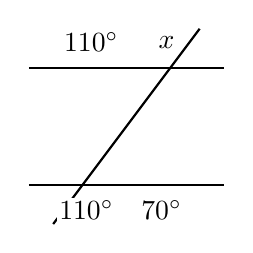
\begin{tikzpicture}[scale=0.62,baseline=(current bounding box.center)]
\draw[thick] (-2,1.2)--(2,1.2);
\draw[thick] (-2,-1.2)--(2,-1.2);
\draw[thick] (-1.5,-2)--(1.5,2);
\node[fill=white,inner sep=1pt] at (-0.72,1.72) {$110^\circ$};
\node[fill=white,inner sep=1pt] at (0.82,1.72) {$x$};
\node[fill=white,inner sep=1pt] at (-0.82,-1.72) {$110^\circ$};
\node[fill=white,inner sep=1pt] at (0.72,-1.72) {$70^\circ$};
\end{tikzpicture}}

\task {Find \mbox{$y$}.\\[0.4em]
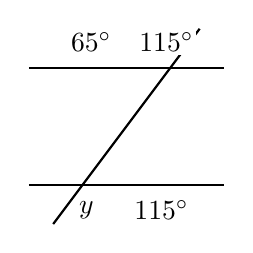
\begin{tikzpicture}[scale=0.62,baseline=(current bounding box.center)]
\draw[thick] (-2,1.2)--(2,1.2);
\draw[thick] (-2,-1.2)--(2,-1.2);
\draw[thick] (-1.5,-2)--(1.5,2);
\node[fill=white,inner sep=1pt] at (-0.72,1.72) {$65^\circ$};
\node[fill=white,inner sep=1pt] at (0.82,1.72) {$115^\circ$};
\node[fill=white,inner sep=1pt] at (-0.82,-1.72) {$y$};
\node[fill=white,inner sep=1pt] at (0.72,-1.72) {$115^\circ$};
\end{tikzpicture}}

\task {Find \mbox{$a$}.\\[0.4em]
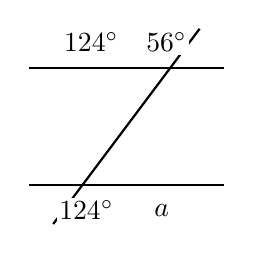
\begin{tikzpicture}[scale=0.62,baseline=(current bounding box.center)]
\draw[thick] (-2,1.2)--(2,1.2);
\draw[thick] (-2,-1.2)--(2,-1.2);
\draw[thick] (-1.5,-2)--(1.5,2);
\node[fill=white,inner sep=1pt] at (-0.72,1.72) {$124^\circ$};
\node[fill=white,inner sep=1pt] at (0.82,1.72) {$56^\circ$};
\node[fill=white,inner sep=1pt] at (-0.82,-1.72) {$124^\circ$};
\node[fill=white,inner sep=1pt] at (0.72,-1.72) {$a$};
\end{tikzpicture}}

\task {Find \mbox{$b$}.\\[0.4em]
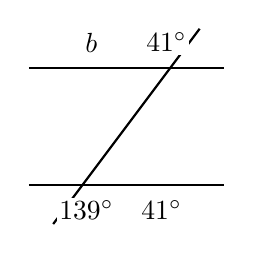
\begin{tikzpicture}[scale=0.62,baseline=(current bounding box.center)]
\draw[thick] (-2,1.2)--(2,1.2);
\draw[thick] (-2,-1.2)--(2,-1.2);
\draw[thick] (-1.5,-2)--(1.5,2);
\node[fill=white,inner sep=1pt] at (-0.72,1.72) {$b$};
\node[fill=white,inner sep=1pt] at (0.82,1.72) {$41^\circ$};
\node[fill=white,inner sep=1pt] at (-0.82,-1.72) {$139^\circ$};
\node[fill=white,inner sep=1pt] at (0.72,-1.72) {$41^\circ$};
\end{tikzpicture}}

\task {Find \mbox{$c$}.\\[0.4em]
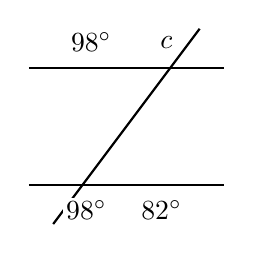
\begin{tikzpicture}[scale=0.62,baseline=(current bounding box.center)]
\draw[thick] (-2,1.2)--(2,1.2);
\draw[thick] (-2,-1.2)--(2,-1.2);
\draw[thick] (-1.5,-2)--(1.5,2);
\node[fill=white,inner sep=1pt] at (-0.72,1.72) {$98^\circ$};
\node[fill=white,inner sep=1pt] at (0.82,1.72) {$c$};
\node[fill=white,inner sep=1pt] at (-0.82,-1.72) {$98^\circ$};
\node[fill=white,inner sep=1pt] at (0.72,-1.72) {$82^\circ$};
\end{tikzpicture}}

\task {Find \mbox{$d$}.\\[0.4em]
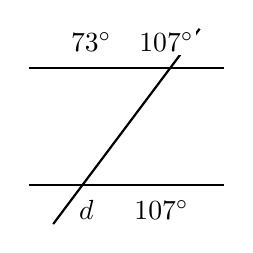
\begin{tikzpicture}[scale=0.62,baseline=(current bounding box.center)]
\draw[thick] (-2,1.2)--(2,1.2);
\draw[thick] (-2,-1.2)--(2,-1.2);
\draw[thick] (-1.5,-2)--(1.5,2);
\node[fill=white,inner sep=1pt] at (-0.72,1.72) {$73^\circ$};
\node[fill=white,inner sep=1pt] at (0.82,1.72) {$107^\circ$};
\node[fill=white,inner sep=1pt] at (-0.82,-1.72) {$d$};
\node[fill=white,inner sep=1pt] at (0.72,-1.72) {$107^\circ$};
\end{tikzpicture}}

\task {Name the rule for the equal angles.\\[0.4em]
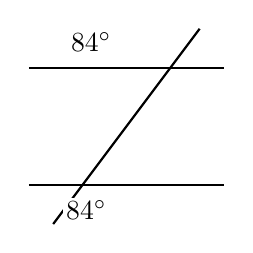
\begin{tikzpicture}[scale=0.62,baseline=(current bounding box.center)]
\draw[thick] (-2,1.2)--(2,1.2);
\draw[thick] (-2,-1.2)--(2,-1.2);
\draw[thick] (-1.5,-2)--(1.5,2);
\node[fill=white,inner sep=1pt] at (-0.72,1.72) {$84^\circ$};
\node[fill=white,inner sep=1pt] at (-0.82,-1.72) {$84^\circ$};
\end{tikzpicture}\\[0.2em]
A. corresponding \quad B. co-interior \quad C. vertically opposite}

\task {Name the rule for the equal angles.\\[0.4em]
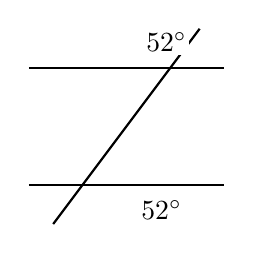
\begin{tikzpicture}[scale=0.62,baseline=(current bounding box.center)]
\draw[thick] (-2,1.2)--(2,1.2);
\draw[thick] (-2,-1.2)--(2,-1.2);
\draw[thick] (-1.5,-2)--(1.5,2);
\node[fill=white,inner sep=1pt] at (0.82,1.72) {$52^\circ$};
\node[fill=white,inner sep=1pt] at (0.72,-1.72) {$52^\circ$};
\end{tikzpicture}\\[0.2em]
A. alternate \quad B. co-interior \quad C. vertically opposite}

\task {Complete the rule: corresponding angles are \mbox{$\underline{\hspace{2cm}}$}.}

\task {Complete the rule: alternate angles are \mbox{$\underline{\hspace{2cm}}$}.}

\task {Complete the rule: co-interior angles add to \mbox{$\underline{\hspace{1.7cm}}$}.}

\task {One angle is \mbox{$118^\circ$}. Find the acute angle made by the same transversal and parallel lines.}
\end{tasks}

\end{document}
